%   Titre de la sous sections
\section{Simuler un dé avec \mbpy}

%   logo mb ou st dans la table des matières
\logo{mbpy}
%\logo{mbot}
%\logo{st}

%
%   style de la page
%   commenter avec % le style non utilisé
\pagestyle{mbpy} %pour microbit
%\pagestyle{mbot} %pour mbot
%\pagestyle{st} %pour ST

\subsection{Description}

\subsubsection{Objectif}


%   bloc de formule
%   sans titre et fond bleu cyan
\begin{formule}
Le but de ce projet est de simuler une expérience aléatoire de lancer d’un dé à 6 faces mais en nous appuyant sur les possibilités offertes par le langage Python.

Ainsi, on ne se contentera pas seulement d'afficher l'issue, mais on montrera comment stocker et traiter facilement les effectifs obtenus. 

Ici, contrairement à l'activité proposée en programmation par blocs, nous suggérons de commencer par simuler l’affichage tel qu’il apparaît sur un vrai dé. Cela permet de réexploiter les listes d’images introduites avec le projet pile ou face.

Cette activité permettra de couvrir de nombreuses capacités du programme de mathématiques de seconde Bac Pro, tant dans le domaine des statistiques que celui de l'algorithmique.

\end{formule}


\subsubsection{Intérêt}


%liste d'arguments
\begin{description}
    \item [expérimenter] En partant d'une modélisation simple, l'élève va pouvoir observer une expérience aléatoire, dont il va facilement pouvoir visualiser et traiter les résultats.
    \item [programmation événementielle] Pour déclencher les tirages et l'affichage, on peut utilise les boutons, mais on peut imaginer utiliser la détection de mouvements. 
    \item [gestion des listes] Même les listes ne font pas partie explicitement des types de données que les élèves sont sensés maîtrisées, il est difficile de s'en passer en programmation. Cependant, il ne semble pas insurmontable de les initier aux principes de création, modification et parcours de listes dans la mesure où l'on retrouve les notions de variables et de boucle for. La majeure difficulté pourrait éventuellement provenir des index.
    \item [programmation fonctionnelle] le calcul des fréquences peut se faire au travers d'une fonction, ce qui permet de scinder la production des données et leur traitement.
    \item [de multiples déclinaisons possibles] Une fois la situation du tirage d'un dé bien établie, il est facilement envisageable d'étendre à d'autres situations : dés non conventionnels, dés multiples.
\end{description}


\subsubsection{Matériel}
\begin{itemize}
%   matériel pour micro:bit
    \item 1 $\times$ \matosMb 
    \item 1 $\times$ IDE programmation python (Mu) \url{https://codewith.mu/} ou interface de programmation ligne \url{https://python.microbit.org/v/1.1}
\end{itemize}



\subsubsection{Remarques}


%   bloc méthode
%   titre + fond bleu
\begin{methode}
    Pour afficher aléatoirement un nombre entier entre 1 et 6, on peut se contenter des 3 lignes ci-dessous.
    \pyfile{13}{17}{./res/mbpy-de.py}
    
    Cette solution peut être envisagée afin de simplifier l'approche, mais la création d'image permet de travailler le repérage et la représentation des nombres, en plus de proposer un affichage plus attrayant.
    
    \begin{enumerate}
        \item \textbf{Initiation - Mise en place du modèle.} \\
            Dans cette activité, il s'agit de proposer aux élèves de créer les images et d'associer l'affichage au résultat d'un tirage aléatoire.
        \item \textbf{Intermédiaire - Enregistrement des résultats.}\\
            L'étape suivante consistera d'une part à stocker les effectifs des différentes issues dans une listes, et d'autre part à afficher les données recueillies.
        \item \textbf{Intermédiaire - Calcul des fréquences}\\
            Le dernier niveau consistera à déterminer les fréquences des issues. Pour cela on utilisera une fonction pour calculer et arrondir.
        
    \end{enumerate}
\end{methode}

%
% activité de niveau initiation
%

%   saut de page
\newpage

%   titre de la sous section
\subsection{Niveau initiation}

\subsubsection{Activité élève}

% commande perso \CARTOUCHE
%   5 paramètres : 
%       * durée
%       * public
%       * travail en maths
%       * travail en sciences
%       * travail en algo
\cartouche
{0,5 h}         %durée
{2de}           %public
{probabilités}        %maths
{}     %sciences
{affichage boucles listes }       %algo


%   petite image de logo qui va
%   se mettre dans le bloc élève
\begin{wrapfigure}[5]{r}{3cm}
    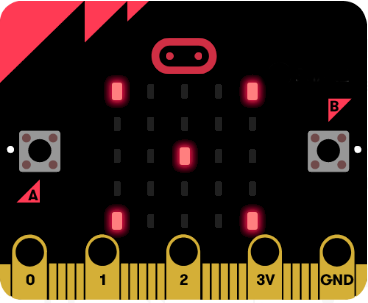
\includegraphics[width=\linewidth]{res/mbpy-de.png}
\end{wrapfigure}

%   bloc élève
%   fond orange
\begin{eleve}    
    \texttt{\textsc{Ta Mission} : Utiliser une carte
    \mb  pour simuler un dé, en utilisant le langage Python.}

Nous utiliserons la bibliothèque \pyline{random} et la fonction \pyline{randint()} pour tirer un nombre entier aléatoirement entre deux bornes. Il faut donc importer un module en plus de microbit:
     \pyfile{1}{2}{./res/mbpy-de.py}
     
Le programme précédent devra être complété avec les éléments suivants :

    \begin{enumerate}
    \item Dans un premier temps nous allons créer les images nécessaires pour afficher les nombres comme sur un vrai dé.
    
    Par exemple le code ci-dessous permet de créer l'image représentant l'issue "cinq".
    \pyfile{9}{9}{./res/mbpy-de.py}
    
    Chaque nombre correspond à une diode, éclairée de 0 à 9.
    
    \item Ces images sont ensuite enregistrée dans une liste :
     \pyfile{23}{23}{./res/mbpy-de.py}
    
    \item Après le démarrage de la boucle \pyline{While True:} on déclenchera le tirage avec le bouton A:  \pyline{button_a.get_presses()}.
    
    \item La première image du tableau \pyline{issues} est numérotée à 0 et la dernière à 5.
    On effectue donc un tirage aléatoire d'un entier entre 0 et 5, puis on demande au \mb d'afficher l'image correspondant à ce numéro.
    
    \pyfile{27}{28}{./res/mbpy-de.py}
    
    \end{enumerate}
    
    Vérifie ton code avec   
\includegraphics[width=0.05\linewidth]{res/check.png} et flash-le sur la carte avec 
\includegraphics[width=0.05\linewidth]{res/flash.png}

    

\end{eleve}



\subsubsection{Notes pour l'enseignant}

%
%   méthode et remarque
%
\begin{methode}
Proposition de résolution :
Il faut bien entendu importer les modules nécessaires
\pyfile{1}{2}{./res/mbpy-de.py}

puis créer les images
\pyfile{5}{10}{./res/mbpy-de.py}


et enfin créer la boucle permettant d'afficher le résultat d'un tirage:
\pyfile{15}{18}{./res/mbpy-de.py}
\end{methode}


\begin{remarque}
   Les deux dernières lignes ne sont pas indispensables, mais elles permettent de mieux différencier les tirages, surtout lorsque l'on tire le même nombre.
\end{remarque}


%
% activité de niveau intermédiaire
%

%   saut de page
\newpage

%   titre de la sous section
\subsection{Niveau intermédiaire}

\subsubsection{Activité élève}

% commande perso \CARTOUCHE
%   5 paramètres : 
%       * durée
%       * public
%       * travail en maths
%       * travail en sciences
%       * travail en algo
\cartouche
{0,5 h}         %durée
{2de}           %public
{probabilités}        %maths
{}     %sciences
{affichage boucles listes }       %algo


%   petite image de logo qui va
%   se mettre dans le bloc élève
\begin{wrapfigure}[5]{r}{3cm}
    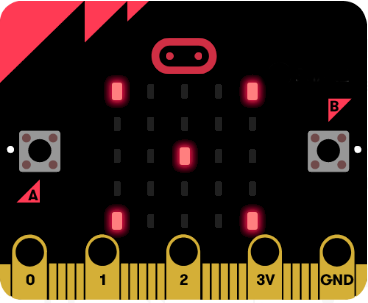
\includegraphics[width=\linewidth]{res/mbpy-de.png}
\end{wrapfigure}

%   bloc élève
%   fond orange
\begin{eleve}    
    \texttt{\textsc{Ta Mission} : Utiliser une carte \mb  pour simuler un dé, et dénombrer les issues en utilisant le langage Python.}

Comme pour l'activité précédente, nous utiliserons la bibliothèque \pyline{random} et la fonction \pyline{randint()}, le programme commencera donc aussi par :
     \pyfile{1}{2}{./res/mbpy-de.py}
     
Le programme de l'activité précédente devra être complété avec les éléments suivants, à vous de déterminer quelle doit être leur position dans le programme :

    \begin{enumerate}
    
    \item Nous allons devoir stocker les effectifs des différentes issues, pour cela il faudra créer un tableau de données que nous initialiserons avec des "0".
    Par exemple :
    
    \pyline{data = [0, 0, 0, 0, 0, 0]}
    
    
    \item Lorsqu'un nombre est tiré, il faudra augmenter l'effectif correspondant de 1. Étant donné que l'on se sert déjà du nombre tiré aléatoirement pour afficher l'image, il n'y a qu'une ligne à rajouter. Par exemple si le tableau s'appelle "data":
    
    \pyline{data[i] = [data[i]+1}
    
    
    \item Pour déclencher l'affichage des effectifs, on utilisera le bouton B :
    \pyline{button_b.get_presses()}
    
    
    \item Pour parcourir le tableau, il faudra faire une boucle \pyline{for ... in ...} sur le tableau et afficher chaque élément du tableau avec \pyline{display.scroll(...)}.
    \pyfile{46}{47}{./res/mbpy-de.py}
    
    \end{enumerate}
    
    
    

\end{eleve}

%   saut de page
\newpage

\subsubsection{Notes pour l'enseignant}

%
%   méthode et remarque
%
\begin{methode}
Proposition de résolution :

Le début du programme est inchangé.

\pyfile{1}{2}{./res/mbpy-de.py}
\pyfile{5}{10}{./res/mbpy-de.py}
\pyfile{23}{24}{./res/mbpy-de.py}

Il faut ajouter l'initialisation du tableau d'effectifs:
\pyfile{35}{36}{./res/mbpy-de.py}

Dans la boucle permettant d'afficher le résultat d'un tirage, il faut inclure l'incrémentation:

\pyfile{37}{43}{./res/mbpy-de.py}

L'affichage des effectifs se fait par parcours du tableau et défilement :
\pyfile{45}{47}{./res/mbpy-de.py}

\end{methode}


\begin{remarque}
   Cette activité étant très guidée, la complexité réside dans le positionnement des instructions proposées dans le programme et dans la compréhension du fonctionnement des listes.
   
   Les listes n'étant pas spécifiquement demandées dans le référentiel de seconde, elles sont à utiliser avec précaution, il est aussi envisageable de créer des variables pour enregistrer l'effectif de chaque issue, mais cela alourdi considérablement le programme.
\end{remarque}



%
% activité de niveau avancé
%

%   saut de page
\newpage

%   titre de la sous section
\subsection{Niveau avancé}

\subsubsection{Activité élève}

% commande perso \CARTOUCHE
%   5 paramètres : 
%       * durée
%       * public
%       * travail en maths
%       * travail en sciences
%       * travail en algo
\cartouche
{0,5 h}         %durée
{2de}           %public
{probabilités}        %maths
{}     %sciences
{affichage boucles listes fonctions}       %algo


%   petite image de logo qui va
%   se mettre dans le bloc élève
\begin{wrapfigure}[5]{r}{3cm}
    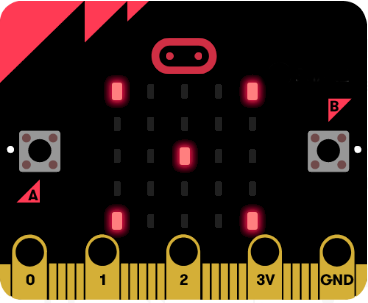
\includegraphics[width=\linewidth]{res/mbpy-de.png}
\end{wrapfigure}

%   bloc élève
%   fond orange
\begin{eleve}    
    \texttt{\textsc{Ta Mission} : Utiliser une carte \mb  pour simuler un dé, et observer la fluctuaion des fréquences en utilisant le langage Python.}

Comme pour l'activité précédente, nous utiliserons la bibliothèque \pyline{random} et la fonction \pyline{randint()}, le programme commencera donc aussi par :
     \pyfile{1}{2}{./res/mbpy-de.py}
     
Le programme de l'activité précédente devra être complété avec les éléments suivants, à vous de déterminer quelle doit être leur position dans le programme :

    \begin{enumerate}
    
    \item Nous allons ajouter une fonction qui nous permettra de calculer les fréquences de chaque issue.
    
    
    \item Pour calculer les fréquences, il nous faut connaître l'effectif total des tirages, et donc pour cela nous devons créer une variable N. 
    
    \item Afin d'obtenir rapidement un grand nombre de tirage, nous allons inclure les instructions liés au tirage dans une boucle de 10 répétitions.
    
    \item Pour déclencher l'affichage des fréquences, on utilisera le bouton B :
    \pyline{button_b.get_presses()}
    
    
    \item 
    
    \end{enumerate}
    
    
    

\end{eleve}

%   saut de page
\newpage

\subsubsection{Notes pour l'enseignant}

%
%   méthode et remarque
%
\begin{methode}
Proposition de résolution :

Le début du programme est inchangé.

\pyfile{1}{2}{./res/mbpy-de.py}
\pyfile{5}{10}{./res/mbpy-de.py}
\pyfile{23}{24}{./res/mbpy-de.py}

Il faut ajouter l'initialisation du tableau d'effectifs:
\pyfile{35}{36}{./res/mbpy-de.py}

Dans la boucle permettant d'afficher le résultat d'un tirage, il faut inclure l'incrémentation:

\pyfile{37}{43}{./res/mbpy-de.py}

L'affichage des effectifs se fait par parcours du tableau et défilement :
\pyfile{45}{47}{./res/mbpy-de.py}

\end{methode}


\begin{remarque}
   Cette activité étant très guidée, la complexité réside dans le positionnement des instructions proposées dans le programme et dans la compréhension du fonctionnement des listes.
   
   Les listes n'étant pas spécifiquement demandées dans le référentiel de seconde, elles sont à utiliser avec précaution, il est aussi envisageable de créer des variables pour enregistrer l'effectif de chaque issue, mais cela alourdi considérablement le programme.
\end{remarque}
